\chapter{Marco Aplicativo}

\section{Implementación de Modelos de Grafos Aleatorios}
Esta sección detalla la implementación de modelos de grafos aleatorios desde cero, sin utilizar librerías especializadas, para incluir en el marco aplicativo de la tesis .


%Para el presente capítulo es necesaria la lectura de los capítulos anteriores por los conceptos que se manejan los cuales son nombrados y fueron introducidos y demostrados anteriormente. El capítulo se centra el desarrollo de los algoritmos junto a su respectivo análisis de complejidad y espacio utilizado.
\subsection{Modelo Erdős-Rényi}
El modelo Erdős-Rényi \( G(n, p) \) conecta cada par de nodos con una probabilidad \( p \) .

\begin{lstlisting}[language=Python]
    import random
    
    def grafo_erdos_renyi(n, p):
    G = {i: set() for i in range(n)}
    for i in range(n):
        for j in range(i + 1, n):
            if random.random() < p:
                G[i].add(j)
                G[j].add(i)
    return G
\end{lstlisting}
\newpage

\begin{figure}
    \centering{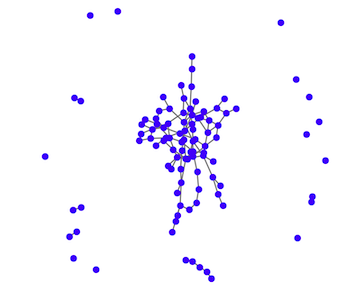
\includegraphics[width=5cm,height=5cm]{images/er1.png}}
\caption{Grafo generado por Erdős-Rényi\\Fuente: Propia}
\end{figure}

\begin{figure}
    \centering{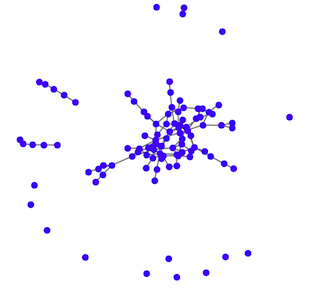
\includegraphics[width=5cm,height=5cm]{images/er2.png}}
\caption{Grafo generado por Erdős-Rényi\\Fuente: Propia}
\end{figure}

\subsection{Modelo Barabási-Albert}

El modelo Barabási-Albert utiliza un mecanismo de conexión preferencial donde cada nuevo nodo se conecta a \( m \) nodos existentes con una probabilidad que es proporcional al grado de los nodos existentes \citep{Barabasi1999} .

\begin{lstlisting}[language=Python]
def grafo_barabasi_albert(n, m):
    G = {i: set() for i in range(m)}
    for i in range(m):
        for j in range(i + 1, m):
            G[i].add(j)
            G[j].add(i)

    # Lista de nodos existentes para elegir segun el grado
    lista_nodos = []
    para i en rango(m):
        lista_nodos.extender([i] * m)

    # Agregar nuevos nodos
    para i en rango(m, n):
        G[i] = set()
        objetivos = set()
        mientras len(objetivos) < m:
            nodo = random.choice(lista_nodos)
            si nodo no en objetivos:
                objetivos.add(nodo)
        para objetivo en objetivos:
            G[i].add(objetivo)
            G[objetivo].add(i)
        lista_nodos.extender([i] * m)
        lista_nodos.extender(objetivos)
    return G
\end{lstlisting}

\begin{figure}[h]
    \centering{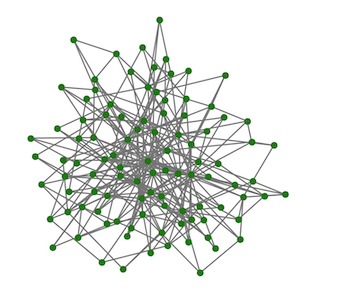
\includegraphics[width=5cm,height=5cm]{images/ba1.png}}
\caption{Grafo generado por Barabási-Albert\\Fuente: Propia}
\end{figure}
\newpage

\begin{figure}[h]
    \centering{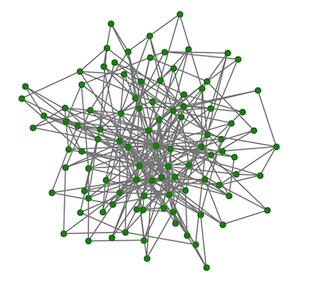
\includegraphics[width=5cm,height=5cm]{images/ba2.png}}
\caption{Grafo generado por Barabási-Albert\\Fuente: Propia}
\end{figure}


\subsection{Modelo Watts-Strogatz}

El modelo Watts-Strogatz comienza con un anillo regular y reconecta cada enlace con una probabilidad \( \beta \) a un nuevo nodo aleatorio para introducir el efecto de mundo pequeño \citep{Watts1998} .

\begin{lstlisting}[language=Python]
def grafo_watts_strogatz(n, k, beta):
    G = {i: set() for i in range(n)}
    para i en rango(n):
        para j en rango(1, k // 2 + 1):
            vecino = (i + j) % n
            G[i].add(vecino)
            G[vecino].add(i)

    para i en rango(n):
        para j en rango(1, k // 2 + 1):
            si random.random() < beta:
                u = (i + j) % n
                v = random.choice(lista(G[i]))
                si u != v:
                    G[i].remove(v)
                    G[v].remove(i)
                    G[i].add(u)
                    G[u].add(i)
    return G
\end{lstlisting}
\begin{figure}[h]
    \centering{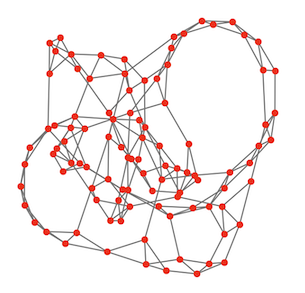
\includegraphics[width=5cm,height=5cm]{images/ws1.png}}
\caption{Grafo generado por Barabási-Albert\\Fuente: Propia}
\end{figure}

\begin{figure}[h]
    \centering{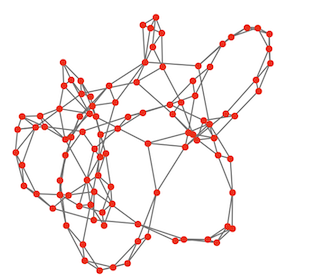
\includegraphics[width=5cm,height=5cm]{images/ws2.png}}
\caption{Grafo generado por Barabási-Albert\\Fuente: Propia}
\end{figure}

\section{Implementación de Funciones}

\subsection{Algoritmo coeficiente de agrupamiento}
\begin{lstlisting}[language=Python]
    # Funcion para calcular el coeficiente de Agrupamiento
    def coeficiente_agrupamiento(G):
        triangulos = 0
        triples = 0
        para u en G:
            vecinos_u = G[u]
            para v en vecinos_u:
                para w en vecinos_u:
                    si v != w y w en G[v]:
                        triangulos += 1
            triples += len(vecinos_u) * (len(vecinos_u) - 1)
        return triangulos / triples si triples > 0 else 0
\end{lstlisting}

\subsection{Algoritmo para calcular Longitud de Caminos Promedio}

\begin{lstlisting}[language=Python]
# Funcion para calcular la longitud promedio del camino mas corto
def longitud_promedio_camino_corto(G):
    def bfs_camino_corto(G, inicio):
        distancias = {vertice: float('infinity') para vertice en G}
        distancias[inicio] = 0
        cola = [inicio]
        mientras cola:
            u = cola.pop(0)
            para v en G[u]:
                si distancias[v] == float('infinity'):
                    distancias[v] = distancias[u] + 1
                    cola.append(v)
        return distancias

    longitud_total = 0
    pares_alcanzables = 0
    para u en G:
        distancias = bfs_camino_corto(G, u)
        para v en distancias:
            si distancias[v] < float('infinity'):
                longitud_total += distancias[v]
                pares_alcanzables += 1
    return longitud_total / pares_alcanzables si pares_alcanzables > 0 else float('infinity')
\end{lstlisting}

\subsection{Algoritmo para calcular la Robustez}
\begin{lstlisting}[language=Python]
    import random

    def calcular_componentes_conexas(G):
        visitado = set()
        componentes = []
    
        def bfs_component(G, inicio):
            cola = [inicio]
            componente = set()
    
            while cola:
                nodo = cola.pop(0)
                if nodo not in visitado:
                    visitado.add(nodo)
                    componente.add(nodo)
                    cola.extend(G[nodo] - visitado)
    
            return componente
    
        for nodo in G:
            if nodo not in visitado:
                componente = bfs_component(G, nodo)
                componentes.append(componente)
    
        return componentes
    
    def robustez_frente_fallos(G, num_eliminaciones):
        nodos = list(G.keys())
        componentes_conexas = []
    
        for _ in range(num_eliminaciones):
            nodo_a_eliminar = random.choice(nodos)
            nodos.remove(nodo_a_eliminar)
            G.pop(nodo_a_eliminar)
            
            for vecino in list(G.values()):
                vecino.discard(nodo_a_eliminar)
    
            componentes_conexas.append(len(max(calcular_componentes_conexas(G), key=len)))
    
        return componentes_conexas
    
    def robustez_frente_ataques(G, num_eliminaciones):
        nodos = list(G.keys())
        nodos_ordenados = sorted(nodos, key=lambda x: len(G[x]), reverse=True)
        componentes_conexas = []
    
        for i in range(num_eliminaciones):
            nodo_a_eliminar = nodos_ordenados[i]
            nodos.remove(nodo_a_eliminar)
            G.pop(nodo_a_eliminar)
            
            for vecino in list(G.values()):
                vecino.discard(nodo_a_eliminar)
    
            componentes_conexas.append(len(max(calcular_componentes_conexas(G), key=len)))
    
        return componentes_conexas
\end{lstlisting}